\newpage
\section*{ANEXO A --- Termo de Ciência e Responsabilidade para o Tratamento dos Dados
Pessoais (SEAD-PI)}

Documento institucional que autoriza o acesso e o tratamento dos dados utilizados nesta
pesquisa, firmado entre a Secretaria de Administração do Estado do Piauí, na condição de
controladora, e o autor, na condição de servidor e pesquisador \cite{seadpi2026termo}. É
reproduzido na íntegra, com tarja sobre os identificadores pessoais --- número de CPF e
matrícula ---, cuja supressão não altera nenhuma das cláusulas.

As cláusulas que condicionam este trabalho são as seguintes.

\begin{citacao}
2.1. O objeto é a concessão de acesso e o tratamento de dados constantes de processos do
Sistema Eletrônico de Informações - SEI, nascidos e movimentados na SEAD-PI no período de
janeiro a dezembro de 2025, para fins acadêmicos e para a realização de estudos e pesquisas
[\ldots]
\end{citacao}

\begin{citacao}
4.4.1. A divulgação acadêmica (nacional ou internacional) limitar-se-á a: nomes de clusters,
exemplos de processos genéricos/sintéticos, métricas agregadas e código-base sem segredos,
sempre anonimizados e previamente aprovados pela SEAD-PI como camada adicional de controle.
\end{citacao}

\begin{citacao}
5.1. A metodologia incluirá etapa de pseudonimização e/ou anonimização dos dados pessoais, de
forma automatizada sempre que identificáveis, antes das fases de clusterização e vetorização.
\end{citacao}

\begin{citacao}
5.2. O grafo inicial de exploração poderá conter dados não anonimizados, cuja etapa integra o
tratamento sob responsabilidade da Controladora, restrita ao ambiente seguro, não constituindo
uso acadêmico autônomo.
\end{citacao}

\begin{citacao}
7.2. A base de dados/grafo derivado de dados públicos será de titularidade da Secretaria de
Administração do Estado do Piauí, com licença de uso acadêmico ao servidor, de acordo com as
diretrizes deste Termo de Responsabilidade.
\end{citacao}

A cláusula 5.1 é a origem do requisito metodológico descrito na seção 3.5: a anonimização não é
uma escolha de projeto, e sim uma condição do instrumento que autoriza o estudo --- razão pela
qual o seu custo em utilidade é medido na seção 4.6 em vez de presumido. A cláusula 4.4.1
submete esta própria divulgação à aprovação prévia da controladora. A cláusula 7.2 delimita o
que pode ser disponibilizado: a metodologia e o código-base são de titularidade do autor
(cláusula 7.1), ao passo que a base derivada é da Secretaria.

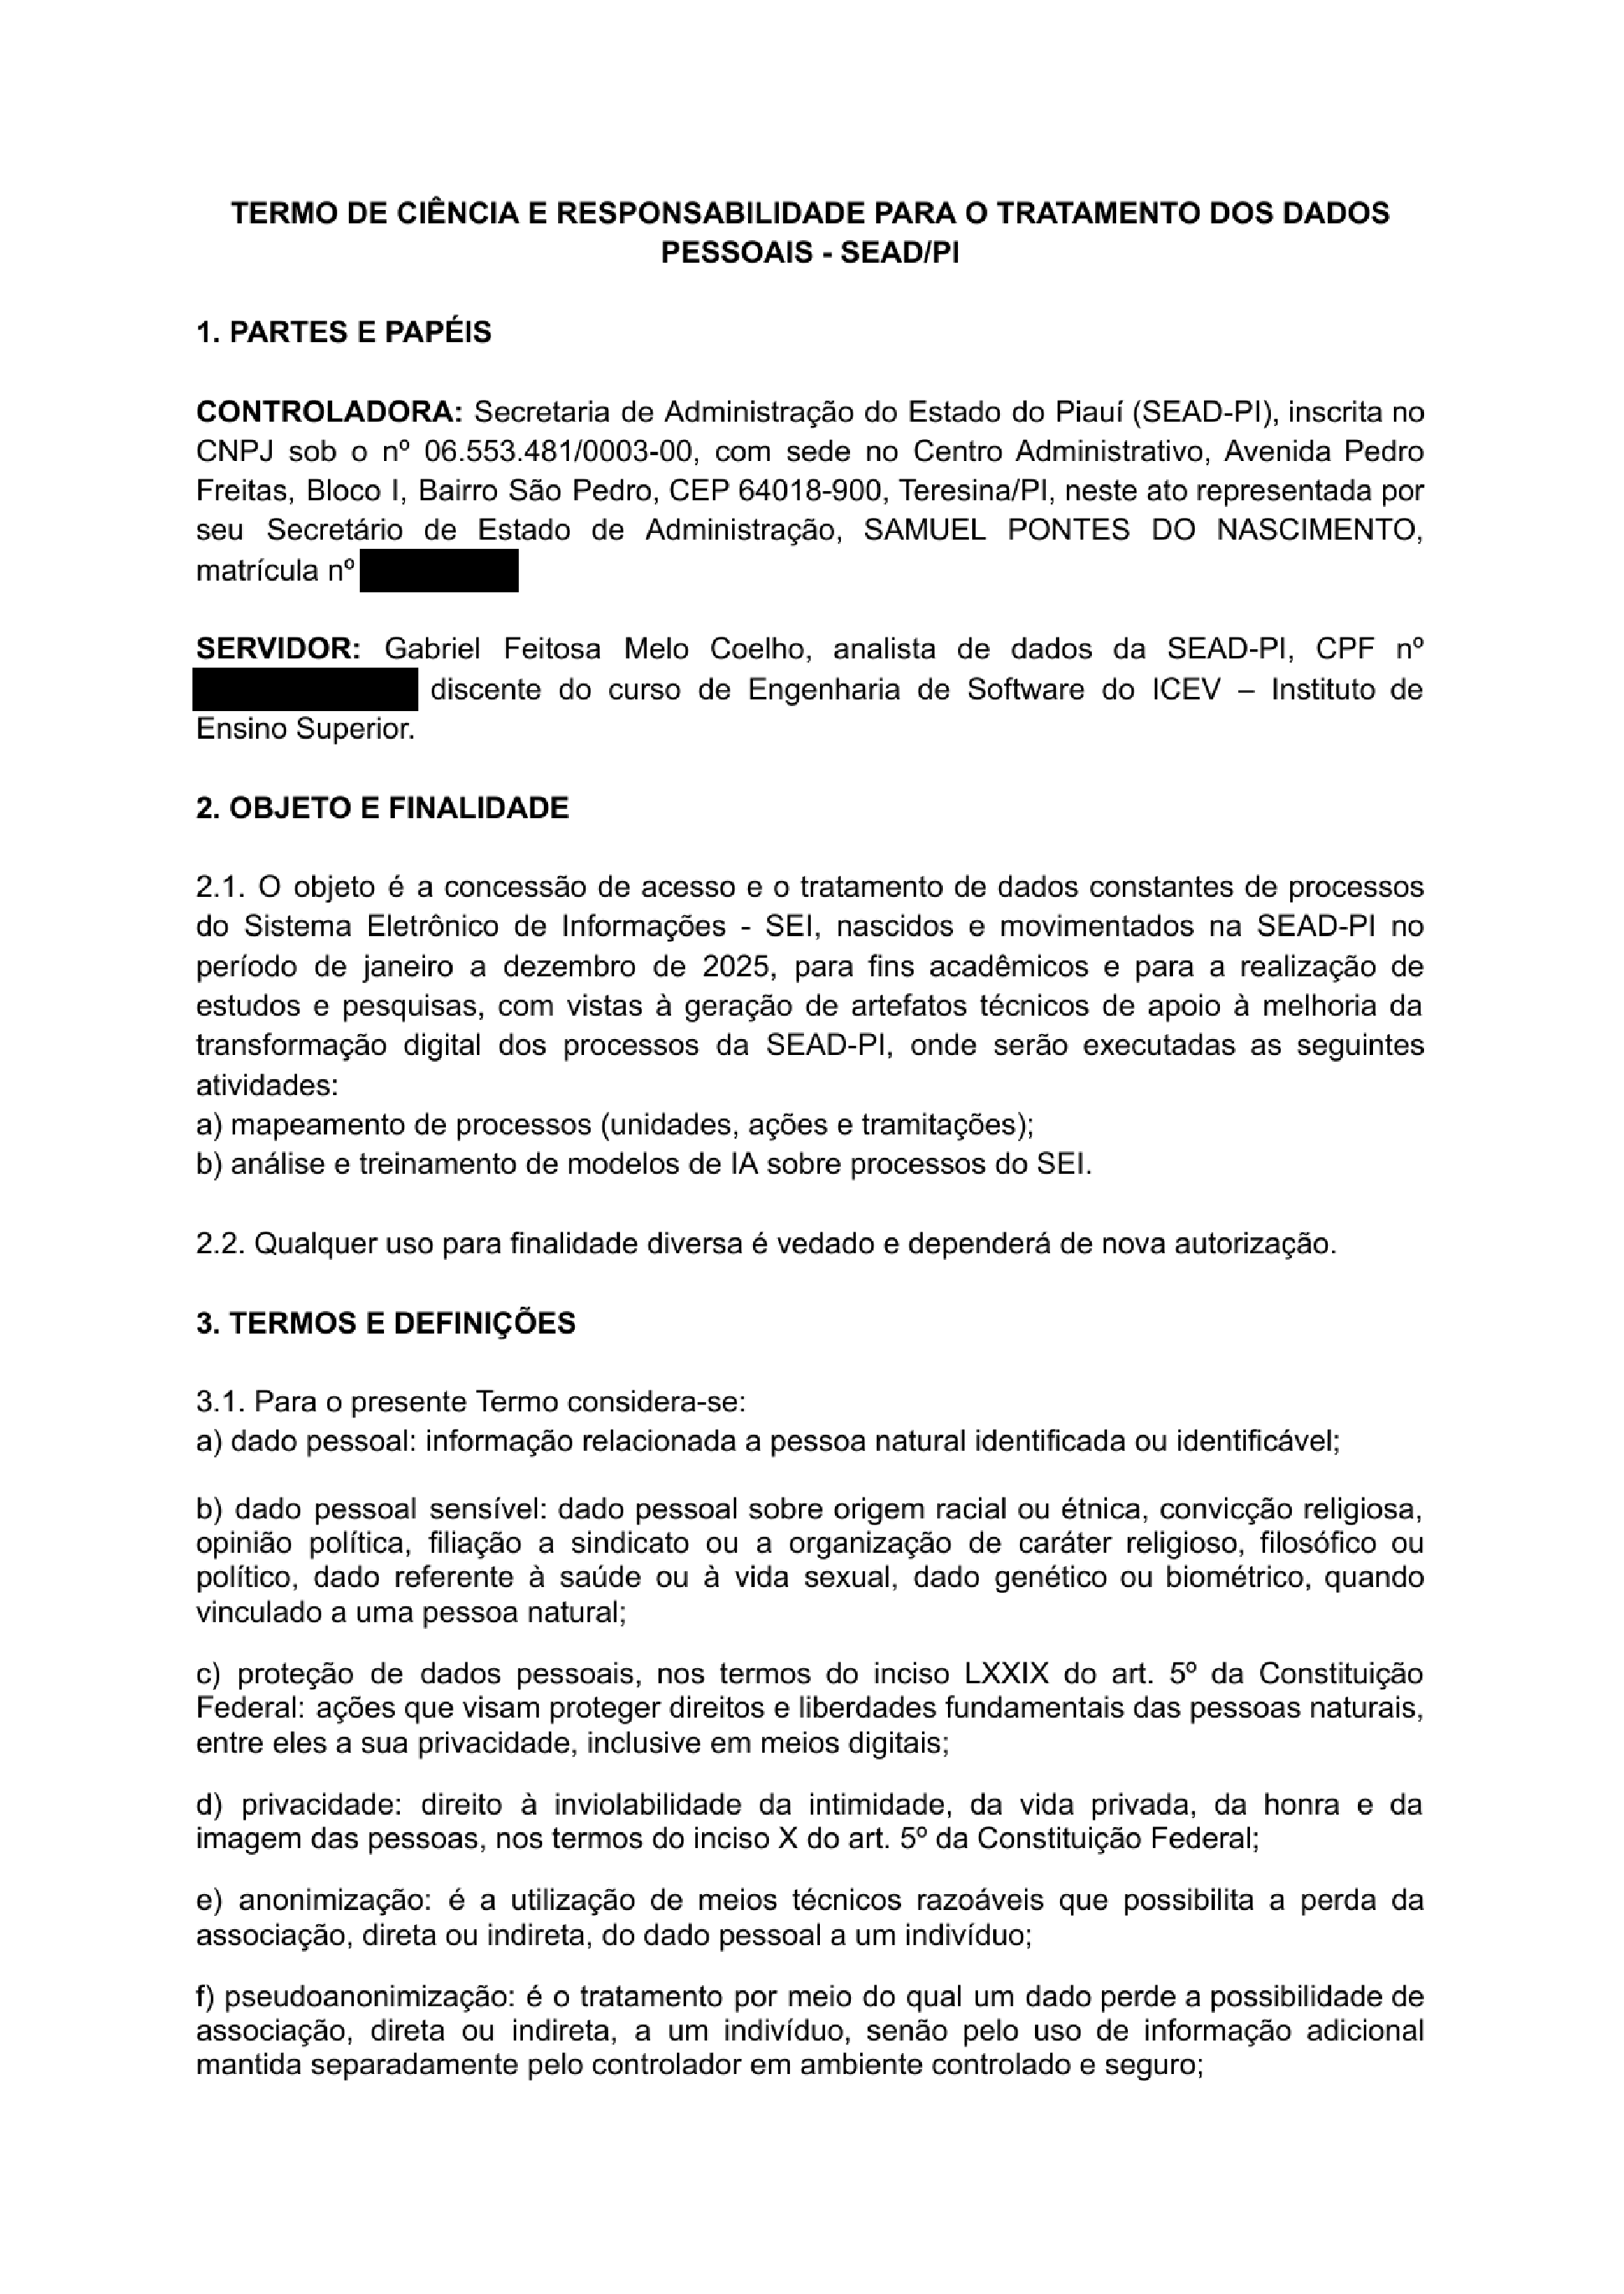
\includepdf[pages=-,frame,scale=0.88,pagecommand={}]{anexos/termo-autorizacao-tarjado.pdf}
